\chapter*{Testing Code Area}
%%%%%%%%%%%%%%%%%%%%%%%%%%%%%%%%%%%%%%%%%%%%%%%%%%%%%%%%%%%%%%%%
\section*{Tables}
\begin{table}[H]
	\caption{Armadillos}
	\label{arm:table}
	\begin{center}
		\begin{tabular}{||l|l||}\hline
			Armadillos & are \\\hline
			our	   & friends \\\hline
		\end{tabular}
	\end{center}
\end{table}
%\clearpage
%%%%%%%%%%%%%%%%%%%%%%%%%%%%%%%%%%%%%%%%%%%%%%%%%%%%%%%%%%%%%%%%
\section*{Figures}
%\vspace*{-3in}
\begin{figure}[H]
%	\vspace{2.4in}
	\caption{Armadillo slaying lawyer.}
	\label{arm:fig1}
\end{figure}
%\clearpage
\begin{figure}[H]
	%%% [H] [ht]
	%%% \captionsetup{justification=raggedright,singlelinecheck=false}
	%%% \flushleft
	%%% \centering
	%%% \begin{center}
	%%%	\vspace{2.4in}
	%%% \includegraphics[scale=0.52]{./image.jpg}
	%%% \end{center}
	%%% \caption{caption}
	%%% \label{label}
\end{figure}
%\clearpage
%%%%%%%%%%%%%%%%%%%%%%%%%%%%%%%%%%%%%%%%%%%%%%%%%%%%%%%%%%%%%%%%
\textbf{Palavras Chave:} \textcolor{blue}{Comportamento Organizacional} \textcolor{blue}{Missão}
%%%%%%%%%%%%%%%%%%%%%%%%%%%%%%%%%%%%%%%%%%%%%%%%%%%%%%%%%%%%%%%%
\begin{figure}[H]
	\centering
	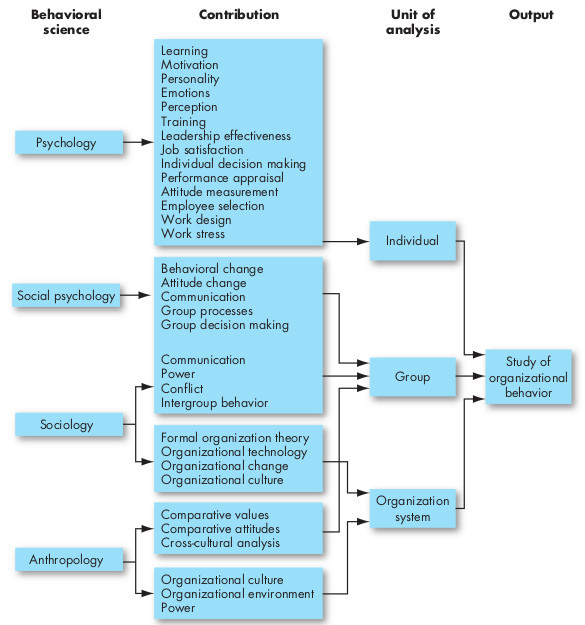
\includegraphics[scale=0.52]{./image/CORGA/OB/OB_contributions.jpg}
	\caption{Contribuições para OB \cite{book_2}}
\end{figure}
%%%%%%%%%%%%%%%%%%%%%%%%%%%%%%%%%%%%%%%%%%%%%%%%%%%%%%%%%%%%%%%%
\begin{figure}[H]
	\begin{minipage}{0.3\linewidth}
		\flushleft
		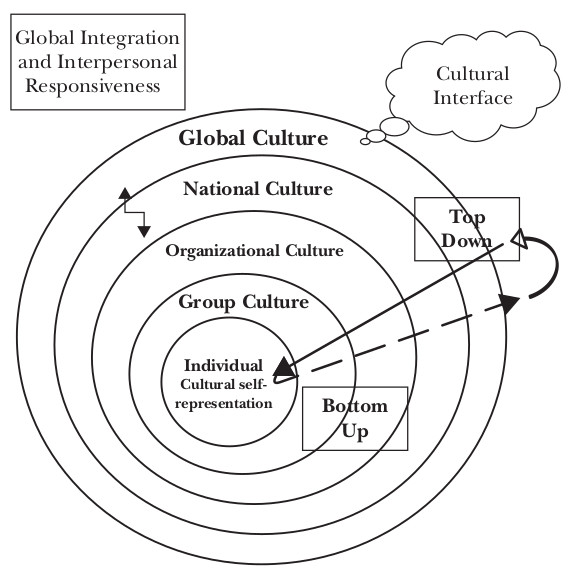
\includegraphics[scale=0.30]{./image/CORGA/OB/OB_MUltilevelmodelCulture.jpg}
	\end{minipage}
	\hspace{1cm}
	\begin{minipage}{0.4\linewidth}
		\flushleft
		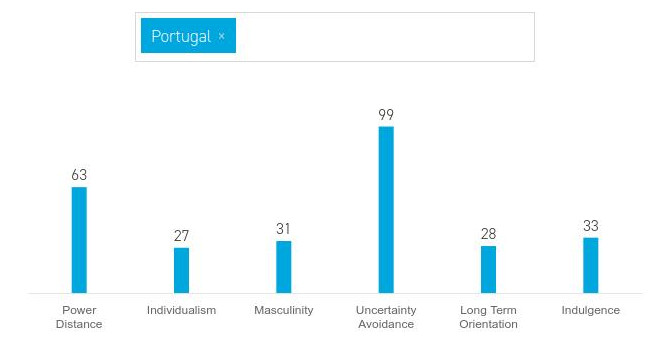
\includegraphics[scale=0.44]{./image/CORGA/OB/Hofstede_pt}
	\end{minipage}
	\caption{Modelo de Multi-níveis \cite{book_11} da cultura e Modelo Hofstede, Portugal}
\end{figure}
%%%%%%%%%%%%%%%%%%%%%%%%%%%%%%%%%%%%%%%%%%%%%%%%%%%%%%%%%%%%%%%%
\begin{figure}[H]
	\flushleft
	\captionsetup{justification=raggedright,singlelinecheck=false}
	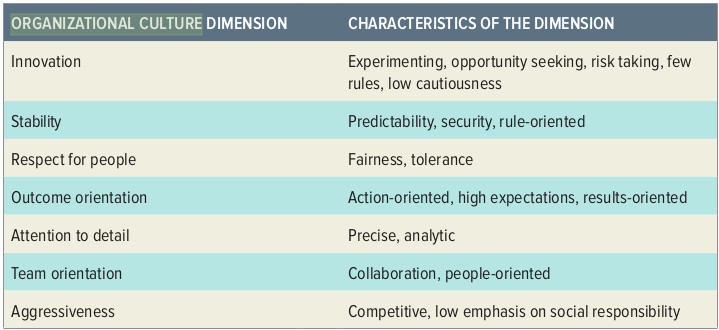
\includegraphics[scale=0.4]{./image/CORGA/OB/OC_Dimensions.jpg}
	\caption{Dimensões da Cultura Organizacional}
	%%%\caption{Dimensões da Cultura Organizacional \cite{book_4}}
\end{figure}\par
%%%%%%%%%%%%%%%%%%%%%%%%%%%%%%%%%%%%%%%%%%%%%%%%%%%%%%%%%%%%%%%%
\qquad A Empresa S.Roque ou ROQ \\
%%%%%%%%%%%%%%%%%%%%%%%%%%%%%%%%%%%%%%%%%%%%%%%%%%%%%%%%%%%%%%%%
\begin{figure}[ht]
	\begin{center}
		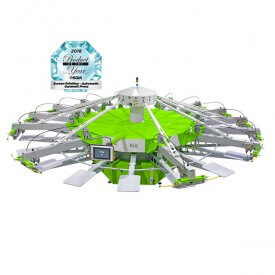
\includegraphics[scale=0.5]{./image/CORGA/ROQ/maquinas/ECO-P18_600x600-2-275x275.jpg}
		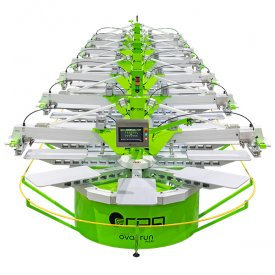
\includegraphics[scale=0.5]{./image/CORGA/ROQ/maquinas/EVO-600x600-275x275.jpg}
		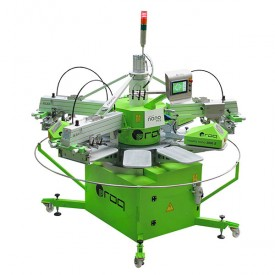
\includegraphics[scale=0.5]{./image/CORGA/ROQ/maquinas/nanop10-275x275.jpg}
		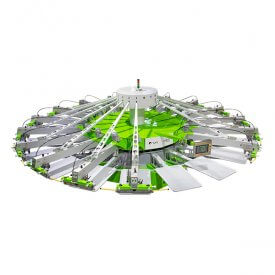
\includegraphics[scale=0.5]{./image/CORGA/ROQ/maquinas/NEXTP18-600x6001-275x275.jpg}
		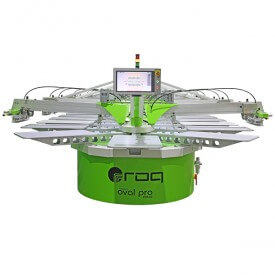
\includegraphics[scale=0.5]{./image/CORGA/ROQ/maquinas/PRO-600x600-275x275.jpg}
		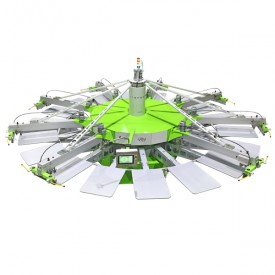
\includegraphics[scale=0.5]{./image/CORGA/ROQ/maquinas/You-600x600-275x275}
	\end{center}
	\caption{Produtos Principais}
\end{figure}
%%%%%%%%%%%%%%%%%%%%%%%%%%%%%%%%%%%%%%%%%%%%%%%%%%%%%%%%%%%%%%%%
\subsection{Valores}
\begin{itemize}
	\setlength\itemsep{-0.3em}
	\item Ação dentro dos princípios morais e éticos da empresa para com os seus stakeholders.
	\item Atuação sempre no interesse dos nossos parceiros de forma a promover a sua satisfação e fidelização.
	\item Excelência conseguida através de trabalho de equipa, competência e responsabilidade.
	\item Qualidade absoluta.
	\item Inovação promovida pelo ADN empreendedor da S. Roque.
	\item Sustentabilidade ambiental e segurança.
\end{itemize}\par
%%%%%%%%%%%%%%%%%%%%%%%%%%%%%%%%%%%%%%%%%%%%%%%%%%%%%%%%%%%%%%%%
\begin{itemize}
	\setlength\itemsep{-0.5em}
	\item \textcolor{purple}{I}nterno
	\begin{itemize}
		\setlength\itemsep{-0.3em}
		\item \textcolor{orange}{S}trength (forças)\\
		- Tem liderança no mercado interno, e reconhecimento internacional\\
		- As maquinas são proprietárias\\
		- Tem um mercado internacional\\
		- Mão de obra qualificada é barata\\
		- Tem um controlo de qualidade\\
		- Dá suporte ao cliente\\
		- Oportunidade de entrar noutros mercados
		\item \textcolor{orange}{W}eakness (fraquezas)\\
		- Mercado saturado internamente\\
		- Localidade de produção isolado\\
		- Dificuldade em obter mão de obra\\
		- Portugal é reconhecido por ter má gestão\\
		- Dificuldade em obter mão de obra qualificada\\
	\end{itemize}
	\item \textcolor{purple}{E}xterno
	\begin{itemize}
		\setlength\itemsep{-0.3em}
		\item \textcolor{orange}{O}pportunity (oportunidades)\\
		- Fácil acesso ao credito\\
		- Inserido num país europeu com mão de obra barata\\
		- Inserido numa sociedade femininista\\
		- Ajudas do estado para o desenvolvimento (ex: programa 2020)\\
		- Tecnologia mais recentes ao dispor\\
		\item \textcolor{orange}{T}hreats (ameaças)\\
		- A competir com mercado internacional mais forte\\
		- Areá têxtil sob ameaça\\
		- Sociedade que evita a incerteza
	\end{itemize}
\end{itemize}
%%%%%%%%%%%%%%%%%%%%%%%%%%%%%%%%%%%%%%%%%%%%%%%%%%%%%%%%%%%%%%%%
\begin{minipage}[t]{.31\linewidth}
	\quad Estilos de Liderança:
	\begin{itemize}
		\setlength\itemsep{-0.3em}
		\item Participativo
		\item Orientado as pessoas\\
		(Liderança de suporte)
		\item Orientado as tarefas\\
		(Liderança Instrumental\\ ou Diretiva\\ ou Transacional)
	\end{itemize}
\end{minipage}
\begin{minipage}[t]{.31\linewidth}
	\quad Tipos de Cultura:
	\begin{itemize}
		\setlength\itemsep{-0.3em}
		\item Inovadora
		\item Competitiva
		\item Burocrática
		\item Comunitária
	\end{itemize}
\end{minipage}
\begin{minipage}[t]{.31\linewidth}
	\quad Medição do Sucesso:
	\begin{itemize}
		\setlength\itemsep{-0.3em}
		\item Satisfação dos Clientes
		\item Taxa crescimento vendas
		\item Cotação no mercado
		\item Vantagens Competitivas
		\item Volume de vendas
	\end{itemize}
\end{minipage}
\vspace{1cm}\\
%%%%%%%%%%%%%%%%%%%%%%%%%%%%%%%%%%%%%%%%%%%%%%%%%%%%%%%%%%%%%%%%
\begin{figure}[H]
	\centering
	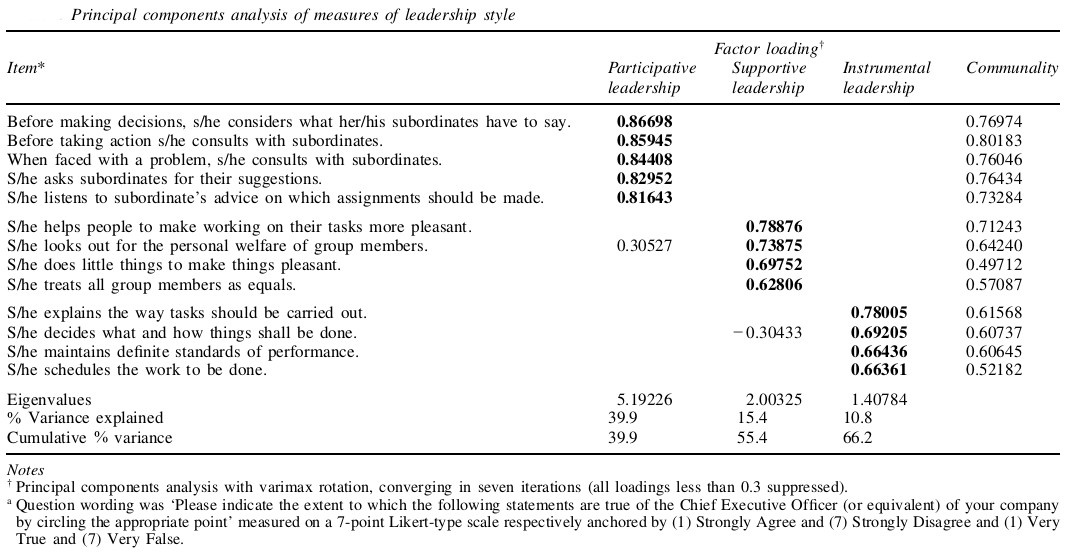
\includegraphics[scale=.5]{./image/CORGA/OB/Leadership.jpg}\\
	\caption{Inquérito do Estilos de Liderança \cite{article_1}}
\end{figure}\par
%%%%%%%%%%%%%%%%%%%%%%%%%%%%%%%%%%%%%%%%%%%%%%%%%%%%%%%%%%%%%%%%
\vspace{1cm}
\begin{figure}[H]
	\centering
	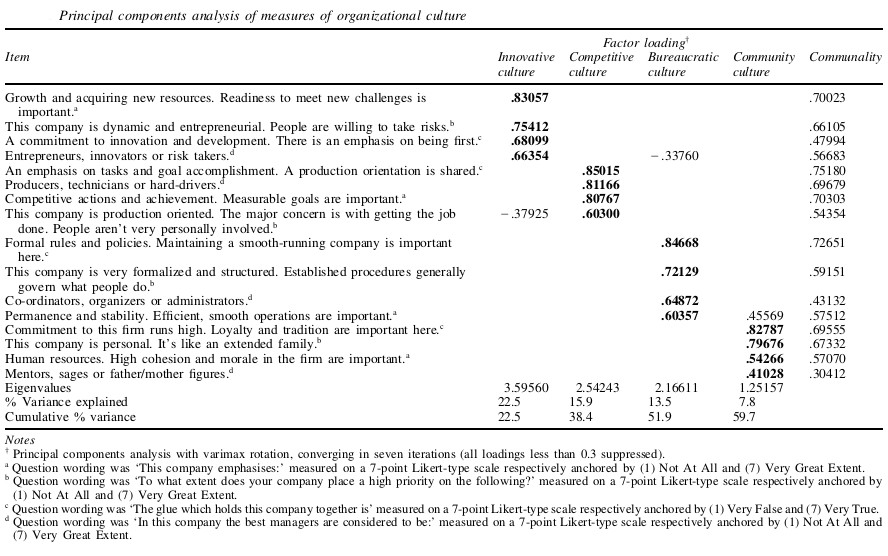
\includegraphics[scale=.6]{./image/CORGA/OB/Culture.jpg}\\
	\caption{Inquérito do tipo de Cultura Organizacional \cite{article_1}}
\end{figure}\par
%%%%%%%%%%%%%%%%%%%%%%%%%%%%%%%%%%%%%%%%%%%%%%%%%%%%%%%%%%%%%%%%
\begin{figure}[H]
	\centering
	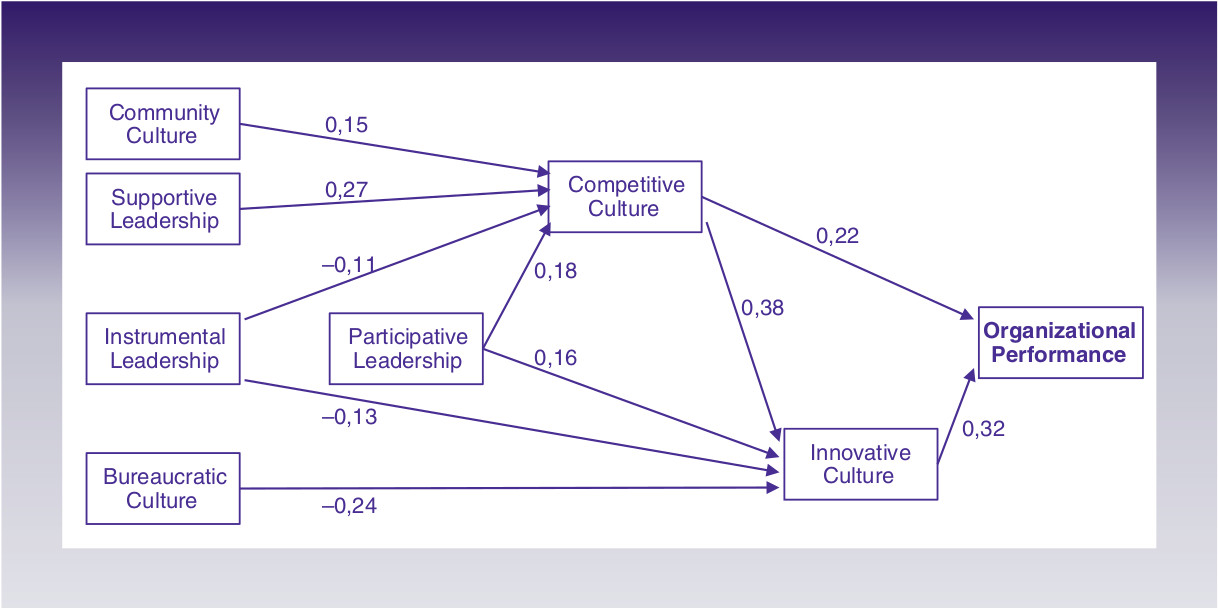
\includegraphics[scale=.35]{./image/CORGA/OB/Ogbonna_Harris.jpg}\\
	\caption{Modelo Ogbonna \& Harris \cite{article_1}}
	\label{Modelo}
\end{figure}\par
%%%%%%%%%%%%%%%%%%%%%%%%%%%%%%%%%%%%%%%%%%%%%%%%%%%%%%%%%%%%%%%%
\begin{table}[h!]
	\begin{adjustbox}{max width=\textwidth}
		\begin{tabular}{ |c|l|c| }
			\hline
			\rowcolor[gray]{0.5}
			Nº & Inquérito & \makecell[l]{Resp \\ 1 \; - \; 7} \\
			\hline
			1. & \makecell[l]{A organização preocupa-se com o crescimento e a aquisição de novos recursos, \\ e procura responder a novos desafios.} & \\
			\hline
			2. & \makecell[l]{A organização é dinâmica e empreendedora. \\ As pessoas estão dispostas a correr riscos.} & \\
			\hline
			3. & \makecell[l]{Existe um elevado empenho na inovação e no desenvolvimento. \\ Procuramos ser os primeiros.} & \\
			\hline
			4. & \makecell[l]{Consideram-se os melhores gestores os que são empreendedores, \\ Inovadores e tomadores de riscos.} & \\
			\hline
			5. & Existe uma elevada ênfase nas tarefas e no alcance de objetivos. & \\
			\hline
			6. & Considera-se que os melhores gestores são produtores e técnicos. & \\
			\hline
			7. & \makecell[l]{A organização valoriza as ações competitivas, \\ o sucesso e o alcance de objetivos mensuráveis.} & \\
			\hline
			8. & \makecell[l]{A organização é orientada para a produção. \\ Uma das maiores preocupações é fazer o que tem que ser feito. \\ Os empregados não estão muito envolvidos do ponto de vista pessoal.} & \\
			\hline
			9. & A organização valoriza muito as regras e as políticas formais. & \\
			\hline
			10. & \makecell[l]{A organização é muito formalizada e estruturada. \\ Os procedimentos estabelecidos orientam o que as pessoas devem fazer.} & \\
			\hline
			11. & Os melhores gestores são considerados os que são coordenadores ou organizadores. & \\
			\hline
			12. & Na organização valoriza-se a permanência, a estabilidade e a eficiência. & \\
			\hline
			13. & Valoriza-se muito a lealdade, a tradição e o empenhamento na organização. & \\
			\hline
			14. & A organização é uma espécie de grande família. & \\
			\hline
			15. & Valoriza-se muito a coesão e os recursos humanos. & \\
			\hline
			16. & \makecell[l]{Considera-se que os melhores gestores são os que atuam como mentores, \\ sábios ou figuras paternais/maternais.} & \\
			\hline
		\end{tabular}
	\end{adjustbox}
\end{table}\par
%%%%%%%%%%%%%%%%%%%%%%%%%%%%%%%%%%%%%%%%%%%%%%%%%%%%%%%%%%%%%%%%
\begin{table}[h!]
	{\small
		\begin{tabular}{|l|c|c|}
			\hline
			& Média do Inquerito & \begin{tabular}[c]{@{}l@{}}Ogbonna \& Harris\\ (2000)\end{tabular} \\ \hline
			\cellcolor[HTML]{C0C0C0}\begin{tabular}[c]{@{}l@{}}Cultura de inovação\\ {[}1-4{]}\end{tabular}     & 5,4 & 4,6 \cellcolor[HTML]{EFEFEF}                                           \\ \hline
			\cellcolor[HTML]{C0C0C0}\begin{tabular}[c]{@{}l@{}}Cultura de Competição\\ {[}5-8{]}\end{tabular}   & 5,3 & 4,2 \cellcolor[HTML]{EFEFEF}                                           \\ \hline
			\cellcolor[HTML]{C0C0C0}\begin{tabular}[c]{@{}l@{}}Cultura Burocrática\\ {[}9-12{]}\end{tabular}    & 4,7  & 4,3 \cellcolor[HTML]{EFEFEF}                                           \\ \hline
			\cellcolor[HTML]{C0C0C0}\begin{tabular}[c]{@{}l@{}}Cultura de Comunidade\\ {[}13-16{]}\end{tabular} & 5  & 4,6 \cellcolor[HTML]{EFEFEF}                                           \\ \hline
		\end{tabular}
	}
\end{table}\par
%%%%%%%%%%%%%%%%%%%%%%%%%%%%%%%%%%%%%%%%%%%%%%%%%%%%%%%%%%%%%%%%
\textcolor{green}{\small [ link: \quad http://www.seg-social.pt/trabalhadores-por-conta-de-outrem ]} \\
\hspace*{.3cm} $635\times(1-0,11)\approx566Eur$,\hspace*{1cm} $635\times(0,3475)\approx220Eur$,\hspace*{1cm} $\frac{635\times14}{12}\times0,65 \approx 482Eur$, \\
%%%%%%%%%%%%%%%%%%%%%%%%%%%%%%%%%%%%%%%%%%%%%%%%%%%%%%%%%%%%%%%%
\begin{figure}[H]
	\centering
	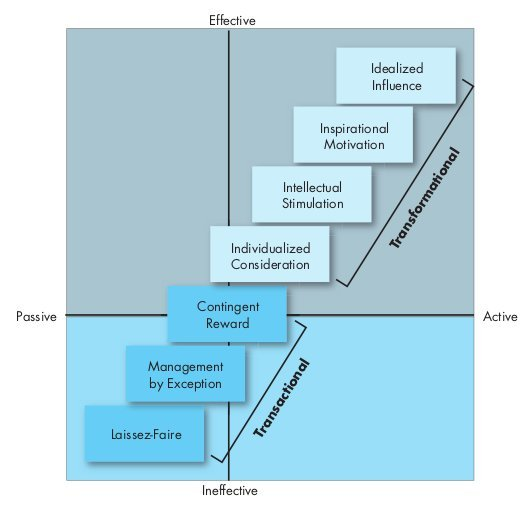
\includegraphics[scale=0.52]{./image/CORGA/Leadership/Leadership_Models.jpg}
	\caption{Modelos da Liderança \cite{book_2}}
	%%% \caption{Modelos da Liderança}
\end{figure}
%%%%%%%%%%%%%%%%%%%%%%%%%%%%%%%%%%%%%%%%%%%%%%%%%%%%%%%%%%%%%%%%
\hspace*{.5cm} - Nunca tiram feriados ou férias\\
\hspace*{.5cm} - Nunca pedem aumentos salariais\\
\hspace*{.5cm} - Nunca custa um cêntimo com folgas de trabalho\\
\hspace*{.5cm} - Nunca fica gripado, problemas de coluna ou dor de dentes\\
\hspace*{.5cm} - Nunca te chateia com situação de desemprego, impostos e segurança social\\
\hspace*{.5cm} - Nunca se cansam de satisfazer \\
%%%%%%%%%%%%%%%%%%%%%%%%%%%%%%%%%%%%%%%%%%%%%%%%%%%%%%%%%%%%%%%%
%\renewcommand{\labelitemi}{$\blacksquare$}
\begin{center}\textbf{\large Competências Consideradas no Estudo OCDE}
%%%\begin{center}\textbf{\large Competências Consideradas no Estudo OCDE \cite{article_1}}
\end{center}
\begin{minipage}[t]{.5\linewidth}
\qquad \textbf{Competências Cognitivas:}
\begin{itemize}
\setlength\itemsep{-1em}
\item Numeração:\\
- Números\\
- Contar\\
- Aritmética\\
\item Literacia:\\
- Falar, Ler, Escrever, Línguas\\
\item Resolução de problemas:\\
- Raciocínio\\
- Lógica\\
- Silogismo\\
- Método Socrático\\
- Critica Interrogativa\\
- etc
\end{itemize}
\qquad \textbf{Competências Socioeconómicas:}
\begin{itemize}
\setlength\itemsep{-1em}
\item Identidade\\
\item Formação Académica:\\
\item Experiência Profissional
\end{itemize}
\qquad \textbf{Personalidade:}\\
\hspace*{1cm}- Facilidade de adaptação\\
\hspace*{1cm}- Facilidade de aprendizagem\\
\hspace*{1cm}- Imaginação\\
\hspace*{1cm}- Estabilidade Emocional\\
\end{minipage}
\begin{minipage}[t]{.5\linewidth}
\qquad \textbf{Competências Operacionais:}
\begin{itemize}
\setlength\itemsep{-0.8em}
\item Gestão e Comunicação:\\
- Planear, Organizar, Controlar, etc\\
- Comunicação formal e informal\\
\item Contabilidade e Vendas:\\
- Marketing Mix\\
- Analise de Parêto\\
- etc\\
\item Organização Pessoal:\\
- Diagrama de Gantt\\
- Analise de Parêto\\
- etc\\
\item Numeração Avançada:\\
- Aritmética, Álgebra, Geometria\\
- Trigonometria, Cálculos\\
- Sistemas Dinâmicos\\
- Estatística\\
- etc\\
\item Tecnologias de informação e comunicação:\\
- Computadores, Telemóvel\\
- Internet, e-mail\\
- Programação\\
- Telecomunicações\\
- etc\\
\end{itemize}
\end{minipage}

%%%%%%%%%%%%%%%%%%%%%%%%%%%%%%%%%%%%%%%%%%%%%%%%%%%%%%%%%%%%%%%%
\section{Plano de desenvolvimento pessoal de competências}
\qquad O meu plano de desenvolvimento pessoal, passa por obter mais formação e aprender com pessoas com mais experiência em diversas áreas, que é exatamente o que estou a fazer frequentando o curso de Engenharia Eletrotécnica e de Computadores no \textcolor{gray}{I.S.E.P}.\\
Esta disciplina em particular é uma forma de poder enriquecer minhas competências e metodologias de Gestão, e perceber as restantes matérias abordadas que compõem o \textcolor{blue}{Comportamento Organizacional}.\\
\begin{minipage}{8cm}
	\textbf{Metodologias da gestão}: \\
	%%%\textbf{Metodologias da gestão}: \cite{book_9}\\
	\\
	\begin{minipage}{3.1cm}
		Instrumental
		\begin{enumerate}
			\setlength\itemsep{-0.3em}
			\item Planear
			\item Organizar
			\item Controlar\\
		\end{enumerate}
	\end{minipage}
	\begin{minipage}{4cm}
		Comportamental
		\begin{enumerate}
			\setlength\itemsep{-0.3em}
			\item Liderança
			\item Comunicação
			\item Motivação
			\item Tomada de decisão
		\end{enumerate}
	\end{minipage}
\end{minipage}
\begin{minipage}{9cm}
\begin{figure}[H]
	\flushleft
	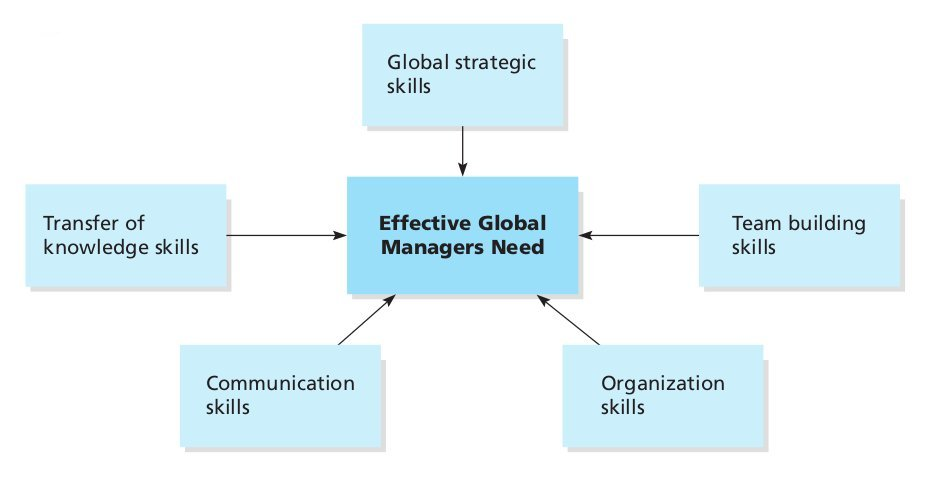
\includegraphics[scale=0.3]{./image/CORGA/Skills/Managerial_Skills_for_the_Global_Marketplace.jpg}
	\caption{Competências de Gestão.}
	%%%\caption{Competências de Gestão. \cite{book_6}}
\end{figure}
\end{minipage}
\\
\\
No entanto por enquanto minha missão é concluir a formação, e ao mesmo tempo melhorar um conjunto de ferramentas e métodos de trabalho para que seja estável e eficaz de forma a poder resolver os problemas que possa ter que enfrentar com facilidade, e eventualmente realizar alguns projetos pessoais. \\
\\
\newpage
\subsection{Análise S.W.O.T Pessoal}
\qquad Neste contexto de plano de desenvolvimento a análise \textcolor{blue}{SWOT} também pode ser uma ferramenta útil de forma a nos indicar qual os comportamentos que poderá ser melhorado ou alterado.
\newline
\newline
\fbox{
\begin{minipage}[t]{\linewidth}
\begin{itemize}
	\setlength\itemsep{-0.85em}
	\item \textcolor{purple}{I}nterno
	\begin{itemize}
		\setlength\itemsep{-0.3em}
		\item \textcolor{orange}{S}trength (forças) \\
		- Numeração, Literacia Bilingue, Resolução de Problemas \\
		- Formação Académica, Experiência Profissional \\
		- Facilidade de Adaptação e aprendizagem, Imaginação \\
		- Gestão e Comunicação, Organização Pessoal \\
		- Numeração Avançada, Tecnologias de informação e comunicação. \\
		- Estabilidade Emocional \\
		- Empatia, Método Cientifico
		\item \textcolor{orange}{W}eakness (fraquezas) \\
		- Contabilidade e Vendas \\
		- Direto, Crítico, Detesto desigualdade e injustiças \\
		- Frontal com contradições \\
		- "Dente por dente e olho por olho" \\
		- Anti-Dogma
	\end{itemize}
	\item \textcolor{purple}{E}xterno
	\begin{itemize}
		\setlength\itemsep{-0.3em}
		\item \textcolor{orange}{O}pportunity (oportunidades) \\
		- Nenhum
		\item \textcolor{orange}{T}hreats (ameaças) \\
		- Cultura Portuguesa \\
		- Sistema Político-Social \\
		- Racismo
	\end{itemize}
\end{itemize}
\end{minipage}
} \vspace{.2cm}

Algumas explicações de personalidade descrevo no caso de quando se diz "dente por dente e olho por olho", muitas das vezes tem interpretação errada, pois concluem que existiria apenas cegos após alguns tempos, mas sendo uma metáfora, sabe-se que ninguém vai andar a cegar uns aos outros sem motivo e são circunstancias de saber individual, mas deve ser percebido no aspeto em que uma pessoa que é honesta merece honestidade, e uma humilde humildade, e pelo verso um mentiroso aldrabado, e assassino deve ser morto, este procedimento leva com que o bem vence sempre, isto é lógico e citações milenares de certa forma condiz neste caso. Que levanta também a questão da veracidade da perceção, na qual muito cuidado é exigido. \\
Dai que certas pessoas quando estão a ser irónicas, acabam dececionados com as reações esperadas, podendo entrar em ciclos viciosos que só vão agravando.\\
\\
Quanto ao método cientifico nos diz que se um acontecimento se repete nas mesmas circunstâncias e nunca se altera é considerado facto ou lei ou teoria, é uma arte de reconhecer padrões. Também nós ensina que os conhecimentos estão sempre abertos ao escrutínio e se houver prova que refuta a teoria esta deixa de o ser, ou seja, é tentar representar a realidade observada por modelos racionais e matemáticos, as ferramentas que estão ao nosso dispor, já que não existe melhor. \\
\\
Acho que esta análise seria mais prudente se fosse feito por uma perspetiva de terceiros, pois nos faria refletir nossas próprias preposições podendo ser reforçado ou até alterado.
\subsection{Curriculum Vitae}
\qquad Curriculum vitae significa "percurso de vida" \; em latim, ao primeiro era pouco conhecido e pouco utilizado, ou reservado apenas a uma fração da população ativa, principalmente aos jovens diplomados ou aos quadros que mudavam de "situação". No entanto os tempos mudaram devido a instabilidade e mudanças que levou a grande procura de novos empregos com muitos candidatos e o principal documento que terá os elementos fundamentais, que conduzem à apreciação e seleção é, sem dúvida, o CV.
%%%\cite{book_12}
O CV é um meio que permite a comunicação, para transmitir tua experiência profissional, tua personalidade na qual deve mencionar tuas motivações e objetivos algo que poderá separar dos restantes candidatos. \\
O Papel do CV serve para sermos selecionados para uma eventual entrevistas de trabalho, e consequentemente obter um acordo ou contrato de trabalho. Este documento é sempre um anexo nas candidaturas por qualquer via de comunicação, seja por e-mail ou contacto direto. \\
O CV em princípio deve conter tua identificação, morada, formação académica e literária, personalidade, experiência profissional e outros assuntos relacionados, ou seja, acaba por ser uma forma de divulgar as tuas competências de forma ordenada e organizada, para ser apelativo deve ser percetível e suscito, na qual só uma observação rápido pode ter uma ideia geral do candidato. \\
\\
\textit{Anexado CV}.
\vspace{1cm}


%%%%%%%%%%%%%%%%%%%%%%%%%%%%%%%%%%%%%%%%%%%%%%%%%%%%%%%%%%%%%%%%
\begin{minipage}{.75\linewidth}
	\begin{tabular}{ |c|c|c|c|c|c|c|c|c|c|c|c| }
		\hline
		\rowcolor[gray]{0.7}
		$h_i$ & CLASSE & MARCA & $n_{i_A}$ & $n_{i_B}$ & $\frac{n_{i_A}}{h_i}$ & $\frac{n_{i_B}}{h_i}$ & $f_{i_A}$	& $f_{i_B}$ & $F_{i_A}$ & $F_{i_B}$ & $e_{i_A}$ \\
		\hline
		$-\infty$ & < 5 & & 0 & 0 & & & & & & & \textcolor{yellow}{1,1812} \\
		\hline
		4 & [5,10[ & 7,5 & 8 & 1 & 2 & 0,25 & 0,0667 & 0,0083 & 0,0667 & 0,0083 & \textcolor{yellow}{5,9871}\\
		\hline
		4 & [10,15[ & 12,5 & 16 & 18 & 4 & 4,5 & 0,1333 & 0,15 & 0,2 & 0,1583 & 18,8942\\
		\hline
		4 & [15,20[ & 17,5 & 40 & 28 & 10 & 7 & 0,3333 & 0,2333 & 0,5333 & 0,3917 & 33,6282\\
		\hline
		4 & [20,25[ & 22,5 & 25 & 41 & 6,25 & 10,25 & 0,2083 & 0,3417 & 0,7417 & 0,7333 & 33,7887\\
		\hline
		4 & [25,30[ & 27,5 & 26 & 22 & 6,5 & 5,5 & 0,2167 & 0,1833 & 0,9583 & 0,9167 & 19,1663\\
		\hline
		4 & [30,35[ & 32,5 & 4 & 8 & 1 & 2 & 0,0333 & 0,0667 & 0,9917 & 0,9833 & \textcolor{orange}{6,1316}\\
		\hline
		5 & [35,40] & 37,5 & 1 & 2 & 0,2 & 0,4 & 0,0083 & 0,0167 & 1 & 1 & \textcolor{orange}{1,1044}\\
		\hline
		$+\infty$ & >40 & & 0 & 0 & & & & & & & \textcolor{orange}{0,1183}\\
		\hline
		& & & n=120 & n=120 & & & & & & & \\
		\hline
	\end{tabular}
\end{minipage}
\newline
%%%%%%%%%%%%%%%%%%%%%%%%%%%%%%%%%%%%%%%%%%%%%%%%%%%%%%%%%%%%%%%%
\begin{minipage}{0pt}
	$$\begin{array}{l | l}
		\text{Média aritmetica dados classificados} & \text{Variância de uma amostra dados classificados} \\
		\overline{x} = \frac{1}{n}\sum_{i=1}^cx_in_i = \sum_{i=1}^cx_if_i & s^2 = \frac{1}{n-1}\sum_{i=1}^c (x_i-\bar{x})^2 n_i
	\end{array}$$
\end{minipage}
\newline
%%%%%%%%%%%%%%%%%%%%%%%%%%%%%%%%%%%%%%%%%%%%%%%%%%%%%%%%%%%%%%%%
\begin{minipage}[!b]{0.40\linewidth}
	\begin{tabular}{ l c c }
		\hline
		Estatística & $X_A$ & $X_B$ \\
		\hline
		Mínimo & 7,5 & 7,5\\
		$Q_1$:$1^o$ Quartil & 17,5 & 17,5 \\
		$m_d$: mediana & 17,5 & 22,5\\
		$Q_3$:$3^o$ Quartil & 27,5 & 27,5 \\
		Máximo & 37,5 & 37,5 \\
		\hline
		$\bar{X}$ : Média & 20,0417 & 21,5417 \\
		$s$ : desvio-padrão & 6,4494 & 6,0909\\
		$m_o$: moda & 17,5 & 22,5\\
		\hline
		Tamanho amostral [$n$] & 120 & 120 \\
		\hline
	\end{tabular}
	\label{Tab:Resultados}
\end{minipage}
\hspace{2cm}
%%%%%%%%%%%%%%%%%%%%%%%%%%%%%%%%%%%%%%%%%%%%%%%%%%%%%%%%%%%%%%%%
\begin{minipage}[!b]{0.40\linewidth}
	\begin{figure}[H]
		\centering
		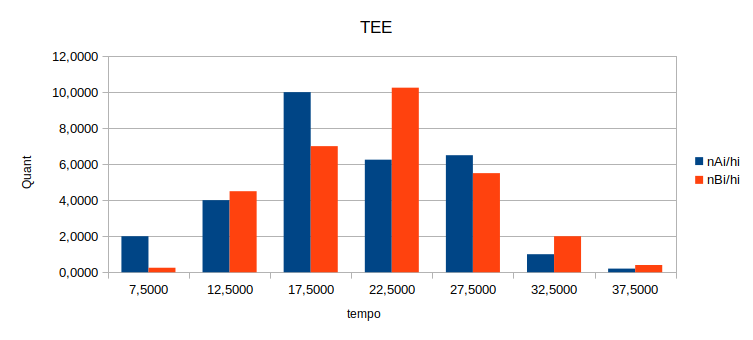
\includegraphics[scale=0.5]{./image/ESTAT/TEE.png}
		\caption{TEE}
		\label{TEE}
	\end{figure}
\end{minipage}
%%%%%%%%%%%%%%%%%%%%%%%%%%%%%%%%%%%%%%%%%%%%%%%%%%%%%%%%%%%%%%%%
$IC_{1-\alpha}=\left[ A, B\right]$ ; para $1-\alpha = 0.95$, $\alpha=0.05$, $\frac{\alpha}{2}=0.025$ \\
Zona critica $Z_c=Z_{1-\frac{\alpha}{2}}=\Phi^{-1}(0.975) \cong 1.96$ \\
$P\left( A \leqslant \mu \leqslant B \right) = 1-\alpha$ \\
$\triangle=Z_c\times\frac{\delta}{\sqrt{n}}$ \\
$A = \bar{x}-\triangle \qquad and \qquad B = \bar{x}+\triangle$ \\
$\therefore$\\
$IC_{A_{0.95}}=\left[ \; 18.8877 \: , \: 21.1956 \; \right]$ \hspace{1cm} and \hspace{1cm} $IC_{B_{0.95}}=\left[ \; 20.4519 \: , \: 22.6314 \; \right]$\\
%%%%%%%%%%%%%%%%%%%%%%%%%%%%%%%%%%%%%%%%%%%%%%%%%%%%%%%%%%%%%%%%
$\left[ \; \mu \; \right]$
%%%%%%%%%%%%%%%%%%%%%%%%%%%%%%%%%%%%%%%%%%%%%%%%%%%%%%%%%%%%%%%%
$\bar{y}_{A_0}$ = 6,6111 \qquad $\bar{y}_{B_0}$ = 7,5111 \qquad $n=90$ \\
$\delta_A$ = 2,3112 \qquad $\delta_B$ = 2,5140 \\
\\
$P(Y_A < 6)=P(Y_A \leqslant 5)=F_{i_B}(5) \cong 0,3677 $  \quad e \quad $P(Y_B < 6)=P(Y_B \leqslant 5)=F_{i_B}(5) \cong 0,2444$ \\
\\
$\hat{P_A}-\hat{P_B} \sim N \left( p_A - p_B ; \frac{p_A\:q_A}{n_A} + \frac{p_B\:q_B}{n_B}\right)$ \hspace{1cm}
$\triangle=z_{(1-\frac{\alpha}{2})} \;\sqrt{\frac{\hat{p_A} \: \hat{q_A}}{n_A}+\frac{\hat{p_B} \: \hat{q_B}}{n_B}}$ \hspace{1cm} $q=(1-p)$ \\
\\
$IC_{97\%}(\hat{P_A}-\hat{P_B})=\left[(\hat{p_A}-\hat{p_B})-\triangle \: ; \: (\hat{p_A}-\hat{p_B})+\triangle \right]$ \\
\\
$\hat{P_A}-\hat{P_B} \sim N \left( 0,1233 \; ; \; 0,02788\right)$ \hspace{1cm}
$z_{(1-\frac{\alpha}{2})}=\phi^{-1}(0,985)=2,1701$ \\
\\
Recorrendo a calculadaora casio $fx-9860GII$ : \\
\\
$\triangle= InvNorm(0.985)\sqrt{\frac{0.3677(1-0.3677)}{90}+\frac{0.2444(1-0.2444)}{90}}\: \cong \:0.3677$
\\
$\therefore$
\\
$IC_{97\%}(\hat{P_A}-\hat{P_B})=\left[ \; (\hat{p_A}-\hat{p_B}) \:-\: 0,3624 \: ; \: (\hat{p_A}-\hat{p_B}) \:+\: 0,3624 \; \right]$ \\
\\
%%%%%%%%%%%%%%%%%%%%%%%%%%%%%%%%%%%%%%%%%%%%%%%%%%%%%%%%%%%%%%%%
\begin{minipage}[l]{0pt}
	$$\left\lbrace\begin{array}{l}
		H_0: \quad \mu_A-\mu_B=0 \\
		\\
		H_1: \quad \mu_A-\mu_B<0
	\end{array}\right.$$
\end{minipage}
%%%%%%%%%%%%%%%%%%%%%%%%%%%%%%%%%%%%%%%%%%%%%%%%%%%%%%%%%%%%%%%%
\begin{minipage}[l]{0pt}
	$$\left\lbrace\begin{array}{c}
		\mu \;=\; 0 \\
		\delta \;=\; s \\
	\end{array}\right.$$
\end{minipage}
\hspace{3cm} $\Longrightarrow$ \hspace{1cm}
\begin{minipage}[l]{0pt}
	\[\bar{X}=\bar{X}_A-\bar{X}_B \quad \backsim N \left( 0\:,\: \frac{\delta_A^2}{n_A}+\frac{\delta_B^2}{n_B} \right) \quad ; \quad \frac{\delta_A^2}{n_A}+\frac{\delta_B^2}{n_B}\;\cong0.6558 \]
\end{minipage}\\
\\
\\
$P(\bar{X}_{H_0} \leqslant C)=0.05 \quad \implies \quad RC_X\left] -\infty \:,\: -1.332 \right] \qquad \bar{x}_A-\bar{x}_B=-1.5 \in RC_X $ \\
\\
%%%%%%%%%%%%%%%%%%%%%%%%%%%%%%%%%%%%%%%%%%%%%%%%%%%%%%%%%%%%%%%%
\begin{minipage}[l]{0pt}
	\[  z_0\:=\: \frac{\bar{x}_A-\bar{x}_B}{\sqrt{\frac{\delta_A^2}{n_A}+\frac{\delta_B^2}{n_B}}}\:\cong\: -1.8523 \qquad
	RC_z \:=\: \left] -\infty \:,\: -1.6448 \right]  \qquad
	pvalue \:=\: P(Z<z_0) \:=\: 0.032 \]
\end{minipage}\\
\\
\\
\hspace*{5cm} \underline{Condição NEE:}\\
\begin{minipage}[l]{0pt}
	$$\left\lbrace\begin{array}{c}
		\mu \;=\; 0 \\
		\delta \;=\; s \\
	\end{array}\right.$$
\end{minipage}
\hspace{3cm} $\Longrightarrow$ \hspace{1cm}
\begin{minipage}[l]{0pt}
	\[ \bar{Y}=\bar{Y_A}-\bar{Y_B} \quad \backsim N \left( 0\:,\: \frac{\delta_A^2}{n_A}+\frac{\delta_B^2}{n_B} \right) \quad ; \quad \frac{\delta_A^2}{n_A}+\frac{\delta_B^2}{n_B} \; \cong 0.1296 \]
\end{minipage}\\
\\
\\
%%%%%%%%%%%%%%%%%%%%%%%%%%%%%%%%%%%%%%%%%%%%%%%%%%%%%%%%%%%%%%%%
$P(\bar{Y}_{H_0} \leqslant C)=0.05 \quad \implies \quad RC_Y\left] -\infty \:,\: -0.5921 \right] \qquad \bar{y}_A-\bar{y}_B=-0.9 \in RC_Y $ \\
\\
%%%%%%%%%%%%%%%%%%%%%%%%%%%%%%%%%%%%%%%%%%%%%%%%%%%%%%%%%%%%%%%%
\begin{minipage}[l]{0pt}
	\[  z_0\:=\: \frac{\bar{y}_A-\bar{y}_B}{\sqrt{\frac{\delta_A^2}{n_A}+\frac{\delta_B^2}{n_B}}}\:\cong\: -2.5 \qquad
	RC_z \:=\: \left] -\infty \:,\: -1.6448 \right]  \qquad
	pvalue \:=\: P(Z<z_0) \:=\: 0.0062 \]
\end{minipage}
\newline
%%%%%%%%%%%%%%%%%%%%%%%%%%%%%%%%%%%%%%%%%%%%%%%%%%%%%%%%%%%%%%%%
\begin{minipage}[l]{0pt}
	$$\left\lbrace\begin{array}{l}
		H_0: X \backsim N (20.0417\;,\;6.4494^2) \\
		\\
		H_1: X \nsim N (20.0417\;,\;6.4494^2)
	\end{array}\right.$$
\end{minipage}\\
%%%%%%%%%%%%%%%%%%%%%%%%%%%%%%%%%%%%%%%%%%%%%%%%%%%%%%%%%%%%%%%%
\hspace*{5cm} \underline{NEE Região B:} \\
%%%%%%%%%%%%%%%%%%%%%%%%%%%%%%%%%%%%%%%%%%%%%%%%%%%%%%%%%%%%%%%%
\begin{minipage}[l]{0pt}
	$$\left\lbrace\begin{array}{l}
		H_0: X \backsim N (7.5111\;,\;2.5140^2) \\
		\\
		H_1: X \nsim N (7.5111\;,\;2.5140^2)
	\end{array}\right.$$
\end{minipage}\\
%%%%%%%%%%%%%%%%%%%%%%%%%%%%%%%%%%%%%%%%%%%%%%%%%%%%%%%%%%%%%%%%
$q_0=\sum_{i=1}^n \frac{(n_i-e_i)^2}{e_i} \;\backsim\; \chi_{(k-m-1)}^2$ \\
\\
$RC_{\chi^2}=\left[ \: InvChiCD(0.05,5) \:,\: +\infty \; \right] \quad \rightarrow \quad RC_{\chi_2}=\left[ \: 11.0705 \:,\: +\infty \; \right]$ \\
\\
$q_0=8.5532$ < 11.0705 \\
%%%%%%%%%%%%%%%%%%%%%%%%%%%%%%%%%%%%%%%%%%%%%%%%%%%%%%%%%%%%%%%%
Distribuição normal Diferença. \\
\begin{minipage}[!b]{0.45\linewidth}
	\begin{figure}[H]
		\centering
		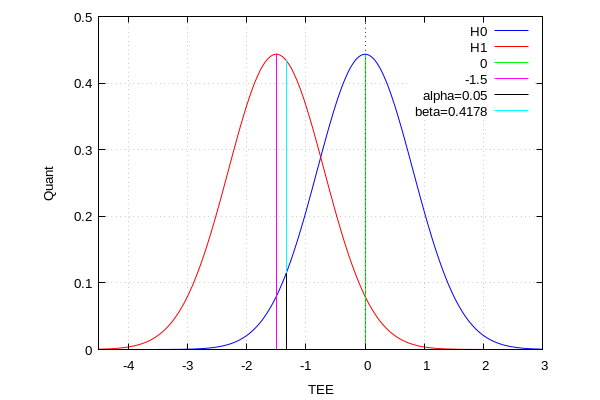
\includegraphics[scale=0.4]{./image/ESTAT/TEE_DIFF.png}
		\caption{TEE Diferênça}
		\label{TEEDIFF}
	\end{figure}
\end{minipage}
\hspace{1cm}
\begin{minipage}[!b]{0.45\linewidth}
	\begin{figure}[H]
		\centering
		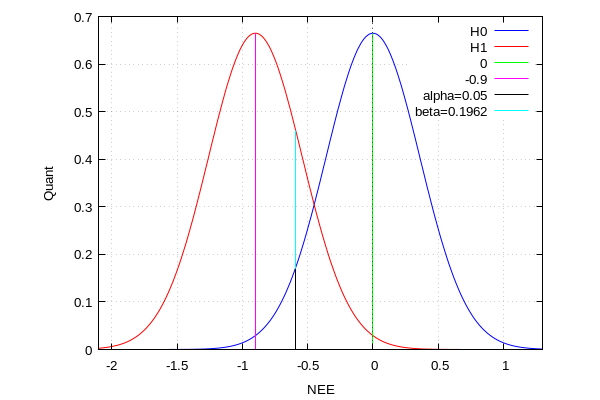
\includegraphics[scale=0.4]{./image/ESTAT/NEE_DIFF.png}
		\caption{NEE Diferença}
		\label{NEEDIFF}
	\end{figure}
\end{minipage} \\
\\
\textbf{Continuação de 3.3} \\
\\
TEE Região A:\\
\begin{minipage}[l]{0pt}
	$$\left\lbrace\begin{array}{l}
		H_0: \bar{X}_{H_0} \backsim N (0 \;,\; 0.6558) \\
		\\
		H_1: \bar{X}_{H_1} \backsim N (-1.5 \;,\; 0.6558)
	\end{array}\right.$$
\end{minipage}\\
%%%%%%%%%%%%%%%%%%%%%%%%%%%%%%%%%%%%%%%%%%%%%%%%%%%%%%%%%%%%%%%%
$\beta=P(Aceitar H_0 | H_0 é Falsa)$ \\
$\beta=(\bar{X}_{H_1} \:>\: -1.332)$	\\
$\beta=NormCD(-1.332,99999999,\sqrt{0.6558},-1.5)=0.4178$ \\
Potência do teste \\
$1-\beta=P(Rejeitar H_0 | H_0 é Falsa)=0.5822$\\
\\
NEE Região B:\\
\begin{minipage}[l]{0pt}
	$$\left\lbrace\begin{array}{l}
		H_0: \bar{Y}_{H_0} \backsim N (0 \;,\; 0.1296) \\
		\\
		H_1: \bar{Y}_{H_1} \backsim N (-0.9 \;,\; 0.1296)
	\end{array}\right.$$
\end{minipage}\\
%%%%%%%%%%%%%%%%%%%%%%%%%%%%%%%%%%%%%%%%%%%%%%%%%%%%%%%%%%%%%%%%
$\beta=P(Aceitar H_0 | H_0 é Falsa)$ \\
$\beta=(\bar{Y}_{H_1} \:>\: -0.5921)$	\\
$\beta=NormCD(-0.5921,99999999,\sqrt{0.1296},-0.9)=0.1962$ \\
Potência do teste \\
$1-\beta=P(Rejeitar H_0 | H_0 é Falsa)=0.8038$\\
%%%%%%%%%%%%%%%%%%%%%%%%%%%%%%%%%%%%%%%%%%%%%%%%%%%%%%%%%%%%%%%%
\begin{minipage}[!b]{0.45\linewidth}
	\begin{figure}[H]
		\centering
		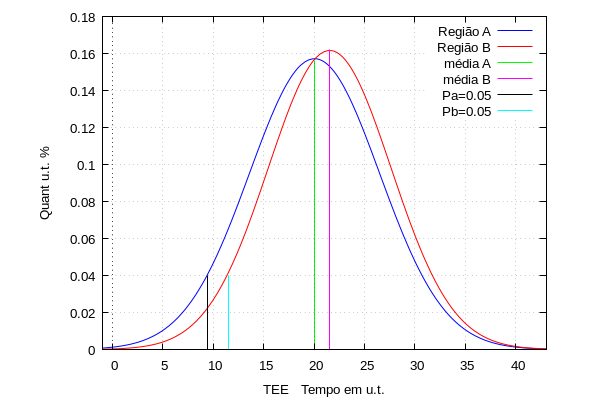
\includegraphics[scale=0.4]{./image/ESTAT/TEE_NORM_DIST.png}
		\caption{TEE Normal}
		\label{TEENORM}
	\end{figure}
\end{minipage}
\hspace{1cm}
\begin{minipage}[!b]{0.45\linewidth}
	\begin{figure}[H]
		\centering
		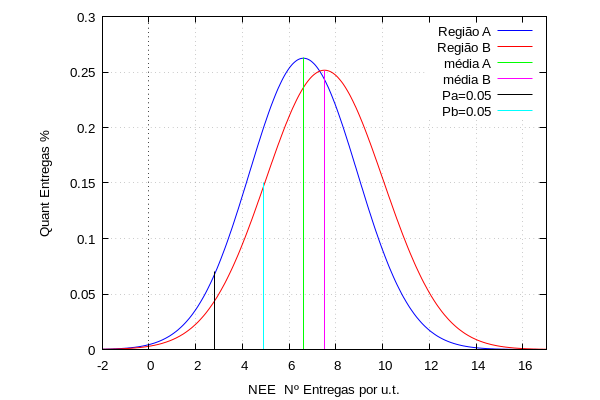
\includegraphics[scale=0.4]{./image/ESTAT/NEE_NORM_DIST.png}
		\caption{NEE Normal}
		\label{NEENORM}
	\end{figure}
\end{minipage} \\
%%%%%%%%%%%%%%%%%%%%%%%%%%%%%%%%%%%%%%%%%%%%%%%%%%%%%%%%%%%%%%%%
\begin{minipage}[!b]{0.45\linewidth}
	\begin{figure}[H]
		\centering
		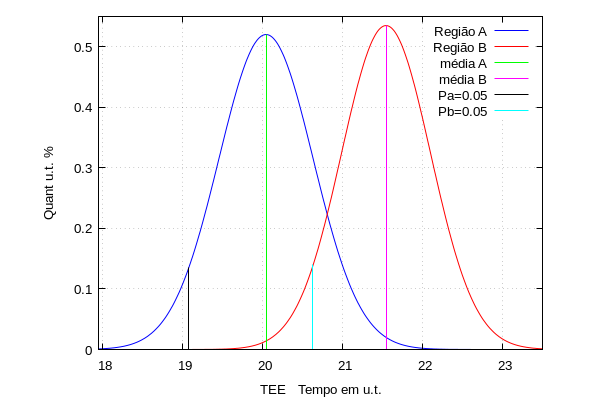
\includegraphics[scale=0.4]{./image/ESTAT/TEE_MEDIA_DIST.png}
		\caption{TEE Normal Média}
		\label{TEEMED}
	\end{figure}
\end{minipage}
\hspace{1cm}
\begin{minipage}[!b]{0.45\linewidth}
	\begin{figure}[H]
		\centering
		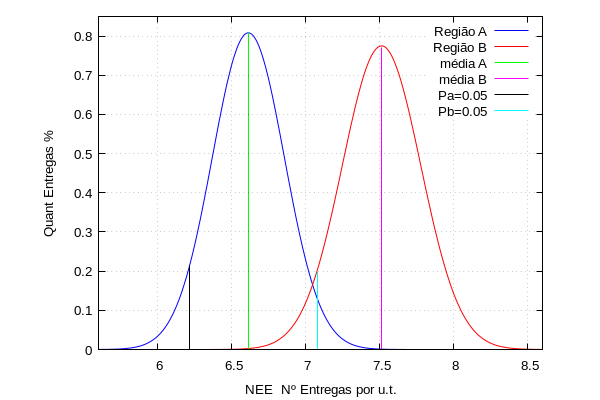
\includegraphics[scale=0.4]{./image/ESTAT/NEE_MEDIA_DIST.png}
		\caption{NEE Normal Média}
		\label{NEEMED}
	\end{figure}
\end{minipage} \\
%%%%%%%%%%%%%%%%%%%%%%%%%%%%%%%%%%%%%%%%%%%%%%%%%%%%%%%%%%%%%%%%
$\chi^2$
%%%%%%%%%%%%%%%%%%%%%%%%%%%%%%%%%%%%%%%%%%%%%%%%%%%%%%%%%%%%%%%%
%%%%%%%%%%%%%%%%%%%%%%%%%%%%%%%%%%%%%%%%%%%%%%%%%%%%%%%%%%%%%%%%
%%%%%%%%%%%%%%%%%%%%%%%%%%%%%%%%%%%%%%%%%%%%%%%%%%%%%%%%%%%%%%%%
%%%%%%%%%%%%%%%%%%%%%%%%%%%%%%%%%%%%%%%%%%%%%%%%%%%%%%%%%%%%%%%%
%%%%%%%%%%%%%%%%%%%%%%%%%%%%%%%%%%%%%%%%%%%%%%%%%%%%%%%%%%%%%%%%
%%%%%%%%%%%%%%%%%%%%%%%%%%%%%%%%%%%%%%%%%%%%%%%%%%%%%%%%%%%%%%%%
%%%%%%%%%%%%%%%%%%%%%%%%%%%%%%%%%%%%%%%%%%%%%%%%%%%%%%%%%%%%%%%%
%%%%%%%%%%%%%%%%%%%%%%%%%%%%%%%%%%%%%%%%%%%%%%%%%%%%%%%%%%%%%%%%
%%%%%%%%%%%%%%%%%%%%%%%%%%%%%%%%%%%%%%%%%%%%%%%%%%%%%%%%%%%%%%%%
%%%%%%%%%%%%%%%%%%%%%%%%%%%%%%%%%%%%%%%%%%%%%%%%%%%%%%%%%%%%%%%%
%%%%%%%%%%%%%%%%%%%%%%%%%%%%%%%%%%%%%%%%%%%%%%%%%%%%%%%%%%%%%%%%
%%%%%%%%%%%%%%%%%%%%%%%%%%%%%%%%%%%%%%%%%%%%%%%%%%%%%%%%%%%%%%%%
%\parte*{The Beginning}
%\chapter*{Tables}
%\chapter*{Figures}
%%%%%%%%%%%%%%%%%%%%%%%%%%%%%%%%%%%%%%%%%%%%%%%%%%%%%%%%%%%%%%%%
\begin{comment}
%%%%%%%%%%%%%%%%%%%%%%%%%%%%%%%%%%%%%%%%%%%%%%%%%%%%%%%%%%%%%%%%
Característica de bons Objetivos\\
- Claros\\
- Concisos\\
- Calendarizados\\
- Atingíveis\\
%%%%%%%%%%%%%%%%%%%%%%%%%
Tipos de organizações\
- Organização privadas com fins lucrativos\\
- Organização privadas sem fins lucrativos\\
- Organização publicas com fins lucrativos\\
- Organização publicas sem fins lucrativos\\
%%%%%%%%%%%%%%%%%%%%%%%%%
tipos de hierarquias\\
tipos de departamentalizações\\
organização por processo\\
%%%%%%%%%%%%%%%%%%%%%%%%%
A divisão do trabalho, permitiu a redução do tempo de aprendizagem, isto é, cada um tem as suas funções, aumentando a produtividade. Cada um executa uma parte das tarefas necessárias a fabricação.\\
%%%%%%%%%%%%%%%%%%%%%%%%%
Gestão:\\ \\
\begin{minipage}{20cm}
\begin{minipage}{5cm}
Instrumentos
\begin{enumerate}
\item Planear
\item Organizar
\item Controlar\\ \\
\end{enumerate}
\end{minipage}
\begin{minipage}{5cm}
Funções
\begin{enumerate}
\item Liderança
\item Comunicação
\item Motivação
\item Tomada de decisão
\end{enumerate}
\end{minipage}
\end{minipage}
%%%%%%%%%%%%%%%%%%%%%%%%%
Cadeia de valor\\
-Atividades principais\\
-Atividades de suporte\\
%%%%%%%%%%%%%%%%%%%%%%%%%
\end{comment}
%%%%%%%%%%%%%%%%%%%%%%%%%%%%%%%%%%%%%%%%%%%%%%%%%%%%%%%%%%%%%%%%
%%%%%%%%%%%%%%%%%%%%%%%%%%%%%%%%%%%%%%%%%%%%%%%%%%%%%%%%%%%%%%%%
%%%%%%%%%%%%%%%%%%%%%%%%%%%%%%%%%%%%%%%%%%%%%%%%%%%%%%%%%%%%%%%%